\chapter{Giriş}

Günümüz akıllı telefonlarının kolay programlanabilirliği, üçüncü parti uygulamalar için etkin dağıtım olanakları ve artan etkili algılama yetenekleri sayesinde, telefonlar insanların davranışlarını takip etmek için etkili birer araç haline gelmiştir. Tüm bu etmenlerin yanı sıra gelişen donanım teknolojisi, telefonları kullanıcısına telefon görüşmesinden daha fazlasını sunan cihazlar haline getirmiştir. Akıllı telefonların sahip olduğu GPS, mikrofon, kamera, ivmeölçer ve jiroskop gibi donanımların sağlamış olduğu veriler sağlık, sosyal medya, taşıma, çevresel izleme ve güvenlik gibi çeşitli uygulamaların geliştirilebilmesini mümkün kılmaktadır. Bu çalışmanın konusu kullanıcıların ulaşım türlerinin akıllı telefonlardaki sensörler aracılığı ile tespit edilmesidir.

İnsanların ulaşım davranışlarının akıllı telefonlar aracılığıyla elde edilmesi birçok alanda kolaylıklar sağlamaktadır. Bu alanlardan bir tanesi de şehir planlamasıdır. Şehir planlaması yapılırken insanlardan toplanan veriler Şekil 1.1'deki gibi internet üzerinden veya telefon yoluyla yapılan anketlerden elde edilmektedir. Planlamacılar elde edilen bu anket verilerinden yeteri kadar memnun olmayabilirler. Bunun nedeni modern şehirler karmaşık ve dinamik bir yapı sergilerken anketlerin sadece tek bir noktada veri toplamasıdır. Ulaşım anketi ile ilgili olarak, insanlar ankette anlattıkları yolculuklarını her zaman tam olarak yapmazlar veya insanlar yaptıkları her yolculuğu ankette bildirmezler. Farklı zamanlarda iki veya daha fazla anket yapılmadıkça insanların yolculuklarındaki değişiklikleri ölçmek zordur. Fakat insanlar bu kadar sık yapılan anket taleplerinden kolayca bıkmaktadırlar. Dahası, tekrar tekrar yapılan anketler pahalı ve zaman alıcıdır.

\begin{figure}[!h]
\centering
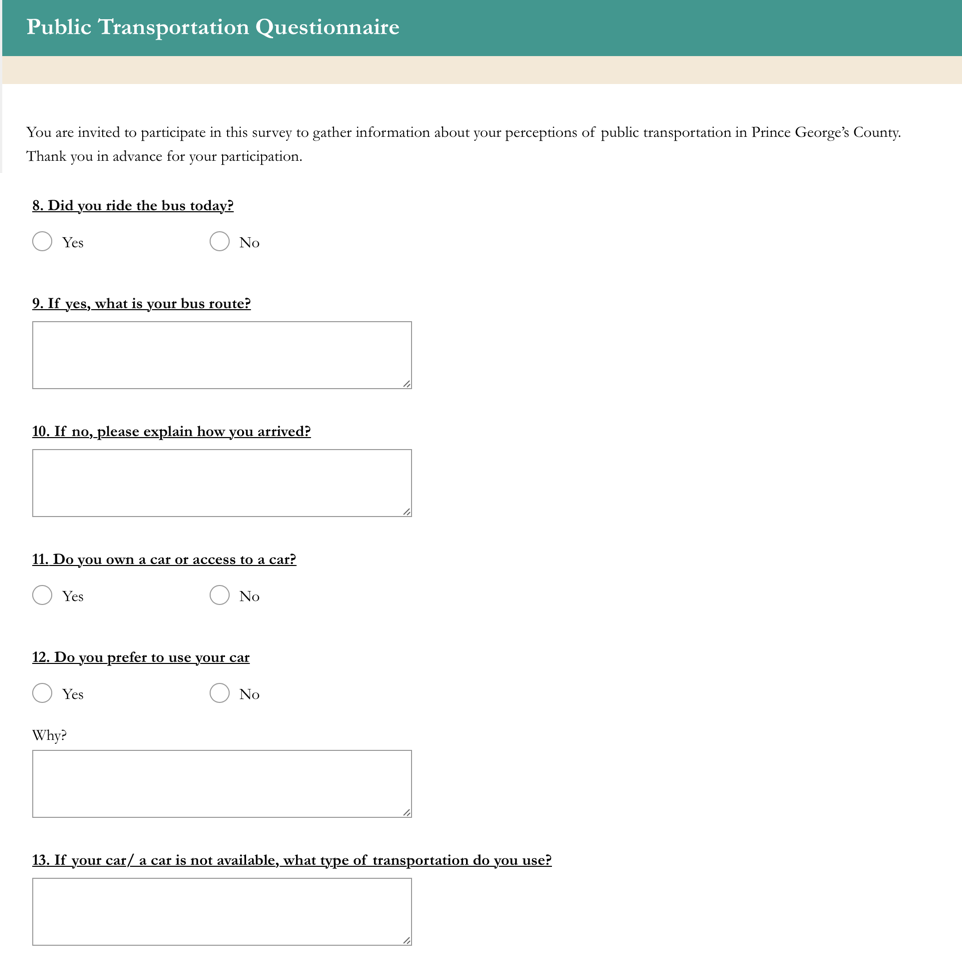
\includegraphics[scale=0.4]{projectChapters/images/Transportation_Survey.png}
\caption{Örnek ulaştırma anketi}
\end{figure}

Ulaşım bilgisinin akıllı telefonlar aracılığıyla otomatik olarak elde edilmesi anketlerin tam tersine çok sayıda insandan kolayca ve zahmetsiz bir şekilde veri toplanmasını sağlamaktadır. Bu yöntem birden fazla insanı gerçek zamanlı izleme fırsatı sunmaktadır. Şehirdeki insanların ulaşım davranışlarının gerçek zamanlı olarak elde edilmesini sağlamaktadır. Bunların yanında şehir planlaması yapan kişiler  bir şehrin hareketlilik modelini çıkarabilmektedirler. Örneğin, bir şehirdeki insanların ortalama hareket mesafeleri elde edilebilmekte, en çok sevilen ulaşım türü belirlenebilmekte ve bu veriler diğer şehirler ile karşılaştırılabilmekte. Şehirdeki insanların belirli saatler içerisinde en çok hangi yolları ve hangi ulaşım araçlarını kullandıkları tespit edilebilir. Bu ve buna benzer bilgiler şehir planlamasında önemli rol oynamaktadır.

Bir diğer önemli kolaylık ise, CO2e (Karbon Ayak İzi) hesaplanması. Endüstriyel Enerji Analizi'ne göre, ulaşım dünya sera gazı emisyonlarının dörtte birini oluşturmaktadir. Kişisel hareketlilik ise toplam ulaşım enerji kullanımının yaklaşık üçte ikisini temsil etmektedir Bu bağlamda, kentin emisyonlarına karşı bireyin kişisel katkısının değerlendirilmesi son derece önemli hale gelmektedir.

Günümüzde kişinin CO2e oranının hesaplanması için Şekil 1.2'de görüldüğü üzeri web uygulamaları kullanılmaktadır. Bu uygulamalar yeteri kadar verimli çalışmamaktadırlar. Bir kişi günlük ortalama CO2e oranını hesaplamak istiyorsa bu web uygulamasına el ile çok fazla sayıda bilgi girmesi gerekmektedir. Bu bilgiler kullanıcı tarafından girildiği için doğru olmayabilir. Ayrıca sistem otomatik çalışmadığı için kullanıcı hesaplama işlemini kendisi düzenli olarak yapması gerekmektedir. 

\begin{figure}[!h]
\centering
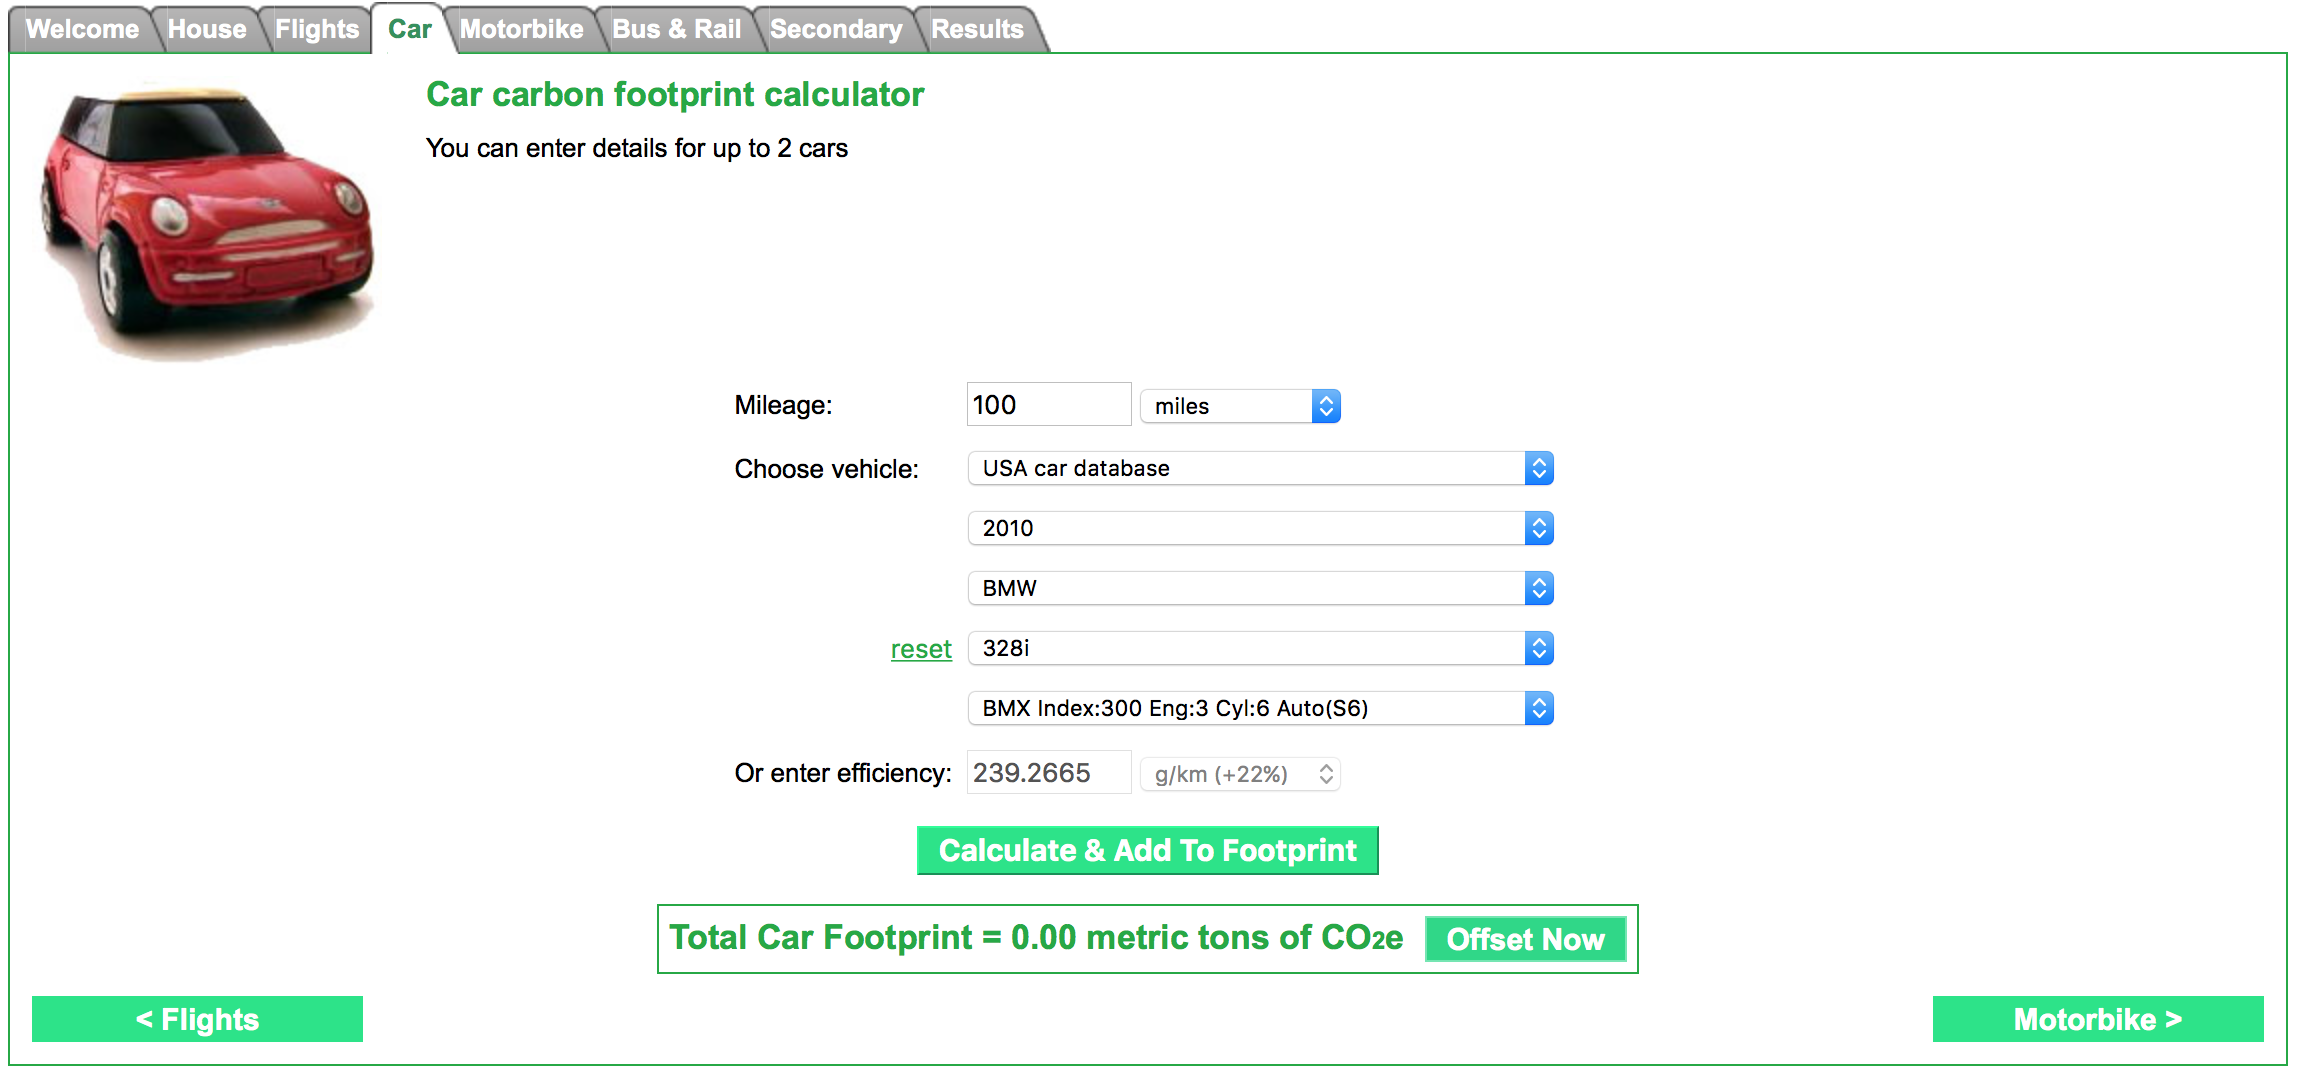
\includegraphics[scale=0.4]{projectChapters/images/CO2_calculator.png}
\caption{Örnek karbon ayak izi hesaplama web uygulamsı}
\end{figure}

Ulaşım türünün otomatik tespiti sayesinde çok sayıda kullanıcının kullandığı vasıta tespit edilebilmektedir. Bu bilginin yanında kullanıcının o anki vasıta ile yapmış olduğu seyehat süresi ve hızı da hasaplanabilmektedir. Tüm bu bilgiler kullanıcının akıllı telefonu cebinde iken elde edilmekte ve otomatik olarak hesaplanmakatır. Bu sayede daha doğru ve etkili bir karbon ayak izi hesabı yapılabilmektedir. Günümüzde bu işlemi yapan CO2GO adında MIT tarafından geliştirilmiş bir uygulama bulunmaktadır. Uygulama Şekil 1.3'de görüldüğü üzere bir çok sensör kullanmaktadır. 

\begin{figure}[!h]
\centering
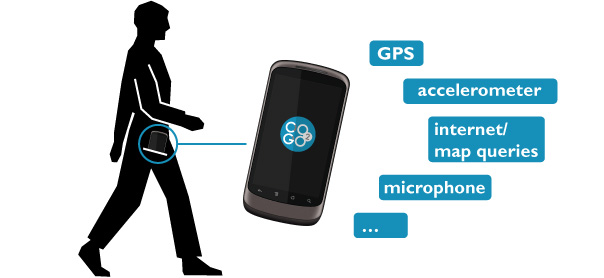
\includegraphics[scale=0.4]{projectChapters/images/sensors.jpg}
\caption{CO2Go uygulaması sensör bilgisi}
\end{figure}

Uygulama, karbon emisyonunun hesaplanmasının yanında kullanıcıların kendilerine ait CO2e oranlarını diğer kullanıcılar ile paylaşmalarına olanak sağlamaktadır. Kullanıcılar bu sayede karbon emisyon oranlarını karşılaştırabilmektedir.

\newpage
Bu proje kapsamında tespit edilmesi beklenen ulaşım türleri Şekil 1.4'de bulunan İstanbul halkının kullandığı toplu taşımalardır. 

\begin{figure}[!h]
\centering
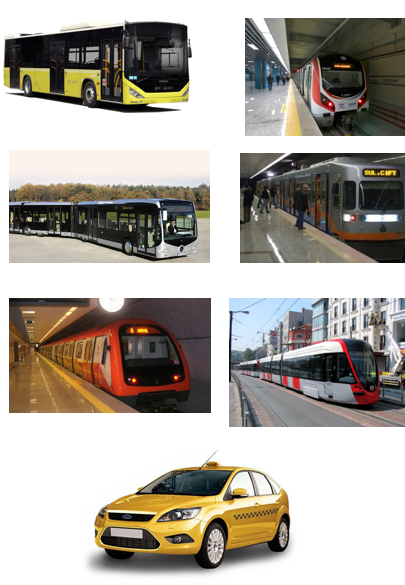
\includegraphics[scale=0.5]{projectChapters/images/Group.png}
\caption{Proje kapsamında tespit edilmesi beklenen vasıtalar}
\end{figure}

Bu toplu taşımalar sırasıyla, otobüs, marmaray, metrobüs, hafif raylı, metro, tramvay ve arabadır. 

Proje kapsamında sensör olarak  şekil 1.5'de gösterilen jiroskop (Gyroscope) ve ivmeölçer (Accelerometer) kullanılmıştır. Soldaki jiroskopu, sağdaki ise ivmeölçeri göstermektedir.

\begin{figure}[!htbp]
\centering
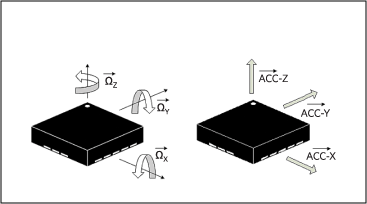
\includegraphics[scale=0.7]{projectChapters/images/acc_and_gyro.png}
\caption{Jiroskop ve İvmeölçer}
\end{figure}

\newpage

İvmeölçer Şekil 1.5’de gösterilen eksenler doğrultusunda akıllı telefona etki eden ivmeyi ölçer. Ham algılayıcı bilgisi ivmeölçerden üç eksende g cinsinden elde edilir. İvmelenme değerlerinin yanında ayrıca zaman bilgisi de elde edilir. Mevcut çoğu ivmeölçer kullanıcı arayüzünde örnekleme hızını ayarlamaya imkân sunmaktadır. Böylece kullanıcı en uygun örnekleme hızını seçebilmektedir. Proje kapsamında kullanılan örnekleme hızı 100Hz olarak belirlenmiştir.
İvmeölçer, akıllı telefon tabanlı eylem tanıma uygulamalarında sıkça kullanılmaktadır. Bu algılayıcının popülerliği konumlandırıldığı cihazın veya taşıyan kullanıcının fiziksel hareketini direkt olarak hesaplayabilmesinden gelmektedir. Örneğin, kullanıcı yürür durumdan zıplar duruma geçerse ivmeölçer sinyallerinin şekli dikey eksende değişir.


Jiroskop ise akıllı telefonun x, y ve z ekseninde yapmış olduğu açısal hızı vermektedir. Jiroskop algılayıcısından elde edilen ham veriler akıllı telefonun üç fiziksel eksen etrafında dönüşünü rad/sn (radyan / saniye) cinsinden bildirmektedir. Karakter yönlendirme yapılan akıllı telefon oyunlarında jiroskop algılayıcısından yararlanılmaktadır. Aktivite tanıma araştırmalarında bu algılayıcı, yön tespitini gerçekleştirmede yardımcı olarak kullanılmaktadır.

Proje raporunun devam eden bölümlerinde sırasıyla ön inceleme, fizibilite ve sistem analizi incelenmektedir.

Ön inceleme bölümü,  projenin yapıldığı alanda daha önceden yapılmış çalışmaların incelenmesini içerir.

Fizibilite bölümü, projenin olabilirliğinin araştırıldığı kısımdır. Projenin zaman planlaması, ekonomik öngörüleri vb. durumları içerir.

Sistem Analizi bölümü ise  sistemin öge ve işlevlerinin ele alınarak ayrıntılı tanımlanmasını içerir. Bu bölümde projenin hedefleri detaylandırılır.
